\documentclass[conference]{IEEEtran}
\usepackage{graphicx}
\usepackage{hyperref}
\usepackage{fixltx2e}
\hyphenation{op-tical net-works semi-conduc-tor}

\makeatletter
\newcommand{\linebreakand}{%
  \end{@IEEEauthorhalign}
  \hfill\mbox{}\par
  \mbox{}\hfill\begin{@IEEEauthorhalign}
}
\makeatother

\begin{document}
    \title{Epidemic Simulation}
    \author{
        \and
        \IEEEauthorblockN{Eeshaan Achar}
        \IEEEauthorblockA{
            Team Lead,\\
            Department of CS\&E (batch of 2021),\\
            JSS Science \& Technology University,\\
            Mysore, India - 570006\\
            Email: eeshaan77@gmail.com
        }
        \and
        \IEEEauthorblockN{Anuj Yadav}
        \IEEEauthorblockA{
            Team Member,\\
            Department of CS\&E (batch of 2021),\\
            JSS Science \& Technology University,\\
            Mysore, India - 570006\\
            Email: yadavanuj952@gmail.com
        }
        \and
        \IEEEauthorblockN{Saurav Kumar}
        \IEEEauthorblockA{
            Team Member,\\
            Department of CS\&E (batch of 2021),\\
            JSS Science \& Technology University,\\
            Mysore, India - 570006\\
            Email: saurav23999ashu@gmail.com
        }
        \linebreakand
        \IEEEauthorblockN{Manjunath Badakar}
        \IEEEauthorblockA{
            Team Member,\\
            Department of CS\&E (batch of 2021),\\
            JSS Science \& Technology University,\\
            Mysore, India - 570006\\
            Email: manjubadakar@gmail.com
        }
        \and
        \IEEEauthorblockN{Dr. H C Vijayalakshmi}
        \IEEEauthorblockA{
            Mentor,\\
            Department of CS\&E (Assoc. Prof),\\
            JSS Science \& Technology University,\\
            Mysore, India - 570006\\
            Email: vijilakshmihc@sjce.ac.in 
        }
    }
    
    \maketitle
    
    \begin{abstract}
        This research paper analyses the results obtained from the simulation of the spread of epidemics over different types of population. This analysis should help increase awareness on the various measures that a society can take to minimise and mitigate the effects of a pandemic. The simulation was done using a software that was built with Python. While not all parameters supported by the simulation software are discussed in this paper, the ones that showed the most interesting results have been picked.
    \end{abstract}

    \section{Introduction}
    An Epidemic is an outbreak of a disease that spreads rapidly and widely. Epidemics such as the Bubonic Plague, Avian flu, H5N1 influenza, H1N1 swine flu, SARS etc. have disturbed human lives for centuries causing massive numbers of deaths and illnesses among people and animals. As the number of urbanized and mobile populations has increased, the possibility of a worldwide pandemic has grown too. The coronavirus pandemic is a testament to the same.\\
    
    Understanding the ways in which diseases propagate has several benefits such as improving healthcare systems, increasing life spans, and reducing the impact of biological warfare. Thus, it is very important for governmental authorities and healthcare agencies to understand how diseases spread and how to limit this spread by selecting the best mitigation and social strategies. Examples of mitigation strategies include vaccination, antiviral treatment, and household prophylaxis. Social distancing strategies include school closure, quarantine, and isolation.\\
    
    Historically, epidemics have been modelled mathematically to understand their dynamics. These models can vary from a few simple equations to complex systems that need to be simulated on supercomputers. The latest advances in high performance computing and computational network science can help epidemiologists develop large-scale high fidelity models of the epidemic spread. These models can help guide public health officials and policy makers in taking appropriate decisions to prevent and control the epidemics.\\ 
    
    This research simulates the spread of a disease on a small population and analyses the results. Based on the disease, and the various measures taken to limit its spread, the parameters would accordingly be tweaked to observe the variations in the result. This paper would also like to summarize the main technical challenges in this field. For the simulation, this research used the basic Susceptible-Infectious-Recovered also called the SIR model. This is a type of compartment model where time is divided into periods and each individual is classified to a particular state in each period. The population is partitioned into three classes: Susceptible (S), Infectious (I), and Recovered (R). A person who becomes infected moves from class S to class I at a rate which depends on the infectiousness of the virus and the prevalence of infection. Infectious individuals who recover from the infection or die from it move to class R.\\
    
    \section{Objectives and Scope}
    Objective is the aim or the final result one wishes to achieve by completing a certain process. The scope of a process defines the limitations that he / she has to face while completing the said process. For a successive process, the objectives have to be achieved within the scope.
        \subsection{Objectives}
            \begin{itemize}
                \item Develop a simulation software with an intuitive UI to enable anyone that is interested to simulate the disease spreading and understand its dynamics.
                \item Simulate the spread of several hypothetical (not necessarily) diseases on several different kinds of population using the said software, and obtain useful information such as the rate of spreading, the rate of recovery of victims, the epidemic duration etc.
                \item Understand and appreciate the effect of various proposed safety measures such as social distancing, hand washing etc. amidst the prevailing coronavirus pandemic, through the simulation of the same.
                \item Understand the various social network models available in the literature, along with their working and relevance.
                \item Appreciate the contributions of various research scholars through their published work, and also propose any improvements if found and feasible.
            \end{itemize}
        \subsection{Scope}
            \begin{itemize}
                \item The simulation will consist of a small sample of population, expected to be around some thousand nodes. This is unlike the real world which consists of over 7 billion humans beings and trillions of other creatures.
                \item Unlike the real world where the behaviour of people vastly differs from each other and is highly unpredictable, the nodes in this simulated world will have a much more defined behaviour.
                \item An epidemic will have varied statistics across varying geography. In this simulation however, these statistics will be fed as parameters and will be constant for the entire population.
                \item There are hundreds of parameters that govern the biological, chemical, and physical dynamics of a disease and its spread through a population. Simulation of all these is impractical, and so this research will be going with a small subset of parameters that are believed the most definitive of an epidemic.
            \end{itemize}
    
    \vspace{0.1in}
    \section{Literature Survey}
    Eleven different research papers were referred to gain useful insights on the spread of various epidemics. These are ``A Social Network Model of the COVID-19 Pandemic" [1] by Zhao, P, ``Simulation of the COVID-19 pandemic on the social network of Slovenia" [2] by Zaplotnik, Z., Gavrić, A., and Medic L., ``SARS: The First Pandemic of the 21st Century" [3] by Cherry, J., and Krogstad, P., ``Strategies for containing an emerging influenza pandemic in Southeast Asia" [4] by Ferguson, N., Cummings, D., Cauchemez, S. and others, ``Mathematical models for devising the optimal Ebola virus disease eradicatio" [5] by Jiang, S., Wang, K., Li, C. and others, ``When individual behaviour matters: homogeneous and network models in epidemiology" [6] by Bansal, S., Grenfell, B. and Meyers, L., ``FluTE, a Publicly Available Stochastic Influenza Epidemic Simulation Model" [7] by Chao, D., Halloran, E. and others, ``Agent-based simulation on avian influenza in Vietnam: Basic characteristics of the epidemic and efficiency evaluation of control measures" [8] by Nguyen, D., Deguchi, H. and others, ``Cholera Epidemic in Haiti, 2010: Using a Transmission Model to Explain Spatial Spread of Disease and Identify Optimal Control Interventions" [9] by Tuite, A., Eisenberg, M. and others, ``Global seasonal occurrence of Middle East Respiratory Syndrome Coronavirus (MERS-CoV) infection" [10] by Nassar, M., Meo, S. and others, ``The effects of border control and quarantine measures on the spread of COVID-19" [11] by Hossain, M. and others. These papers helped this research to analyse the different parameters that affect an epidemic and which one of these should be incorporated in the simulation so that it can closely resemble a real world epidemic. In addition the the papers, the YouTube videos ``Exponential growth and epidemics" [12] and ``Simulating an epidemic" [13] by Sanderson, G., and ``Social Networks" [14] by Iyengar, S., also greatly helped. Lastly, the articles ``Why outbreaks like coronavirus spread exponentially, and how to “flatten the curve”" [15] by Stevens, H., and ``Outbreak" [16] by Simler K., were also contributing.\\
    
    One of the important papers which can be thought as the motivation for this research was ``A Social Network Model of the COVID-19 Pandemic" [1] by Pei Jun Zhao, Harvard T.H. Chan School of Public Health. It provides a conceptual framework to analyze the COVID-19 pandemic on the level of individuals, that can be used to predict the influence of collective social behavior on overall pandemic trajectories. It shows the importance of social distancing, and the message that to contain the epidemic, every member of the public plays a crucial part in breaking the chain of transmission. The social network model of COVID-19 transmission is expandable and extendable. This paper provided a simplified version using population averages for parameters. Another important paper that this research referred was ``Simulation  of  the  COVID-19  pandemic  on  the  social  net-work  of  Slovenia" [2] by Žiga Zaplotnik and others. In this paper, the researchers the social network consisted of more than 2 million nodes, each representing an inhabitant of Slovenia. The nodes were organised and interconnected according to the real household and elderly-care center distribution, while their connections outside these clusters were semi-randomly distributed and undirected. This research specifically focused on the simulation aspect, which was in line with what this research had intended to do. Apart from these (and other papers mentioned under references), there this researchre also two videos [12, 13] by Grant Sanderson, in his YouTube channel ``3Blue1Brown", which explained in great detail using simple terms about the various parameters associated with an epidemic, and also its nature.\\
    
    This research also found out about one of the important mathematical terms used to determine whether an epidemic is about to occur or the disease will diminish, and that is the basic reproduction number, R\textsubscript{0}. R\textsubscript{0} is an indicator, and is defined as the expected number of new infections caused by a single infection in a population where all individuals are susceptible. A value equal to 1 means that the disease is neither dying out nor will the cases rise, as one infected person just transmits his disease to another person. A value greater than one indicates the number of cases will grow and a value less than one indicates the disease will die out. While there are a couple of different ways to calculate R\textsubscript{0}, the following formula is one of the most intuitive: \[R_0 = nTP\] Here `n' is the average contacts made by an individual of the population in a day, `T' is the average duration of the disease, and `P' is the probability of infection. Now as per the definition, to calculate R\textsubscript{0}, there is a need of an unaffected population which means it can't be calculated on a daily basis. For this reason, this research has gone with something known as the effective reproduction number, `R' that eliminates the said clause, and so can be used to analyse the output of the simulation.\\
    
    \section{Work}
    This academic research was conducted as part of a bachelor's program. In the month of November a meeting was carried out to decide upon the problem statement to be ``Epidemic Simulation" in the light of the ongoing pandemic. In the next few days, there were further discussions and the scope and objectives of the research was narrowed down based on the time available, as well as the skills of the researchers. It was decided that the research would be conducted in two phases. The first phase would include the development of a simulation software that would enable this research to simulate the spread of a disease over a population. The second phase would include the actual testing and analysis using the developed software in order to understand the disease dynamics with respect to its own parameters such as infection probability, average infection duration, etc. as well as societal parameters such as social distancing.
    \subsection{Software Modules}
    This research has divided the whole operational process into four modules which are are:\\
        \subsubsection{Initializer Module}
			This module is responsible for generating a graph using NetworkX. The graph, whose structure is defined through the given inputs, represents the population of a city, with the nodes and edges representing people and the physical connectedness among them respectively. The graph (as a whole), nodes, and edges contain parameters defined through the input, and these will be used during the simulation. This module also sets up a few other things such as seeding the randomizer, that are necessary for the simulation.\\
		\subsubsection{Contaminator module}
			This module is responsible for simulating the spread of the defined disease over the population. It uses BFS to do so, however with slight changes. Each outer BFS loop represents a day for the population, and so in order to provide each person with the same probability of infecting others, the queue is shuffled each day. Moreover, unlike traditional BFS, here the nodes aren't removed from the queue after processing, instead are retained until it either dies or recovers from the disease. During the simulation it considers the various input factors to progress until the epidemic is over. In the end it returns the SIR statistics of each day.\\
		\subsubsection{Analyzer Module}
		    This module is responsible for performing analysis using the SIR statistics obtained from the contaminator module. To do so, it first runs the simulation using the said module. Then, it plots three graphs, one for the SIR statistics, one for the total infections until date, and one for the new infections each day. The latter two are also plotted based on the same SIR statistics. Finally, it stores the graphs as a PNG image and returns the filename, along with the peak active cases of the infection and the total duration of the epidemic during the simulation.\\
		\subsubsection{Server Module}
			This module is responsible for accepting the inputs from the user through the UI, constructing a simulation instance using the constructor module, using the analyzer module to run the simulation and get the results, and then sending the results back to the user in the UI. It is a standard Flask module that converts the Python scripts to a WSGI application.
    \subsection{Testing and analysis}
    The final simulation was tested by making several changes in various parameters and combination of parameters, and the results for the respective change were compared against the effect these parameters would have caused in the real world. This research saw that the overall results corresponding to these changes were quite comparable to how an epidemic would behave in a real life situation.\\

    \section{Results}
    The simulation works by taking values for the various parameters, and produces a graphical representation of different observations obtained.
    \subsection{Inputs}
        Following are the simulation parameters that the software takes as inputs to the simulation:
        \begin{itemize}
            \item Population i.e the number of nodes in the graph
    		\item Community centres i.e the minimum number of nodes that need to be connected to at least a tenth of all the nodes
    		\item Average number of friends that an individual has i.e. average degree of nodes
    		\item Quarantine strictness when someone is quarantined
    		\item Quarantine probability when a person is found to be infected
    		\item Total hospital beds available
    		\item Average immunity of the population, with 1 and 0 being 100\% and 0\% immune to the disease
    		\item Immunity variation*
    		\item Average social distance (in metres) maintained by the people
    		\item Social distance variation*
    		\item Average adherence to safety measures by the people in the range 0 and 1
    		\item Adherence to safety measures variation*
    		\item Average travel probability of the people in the range 0 and 1
    		\item Travel probability variation*
    		\item Travel ban strictness imposed by the authorities
    		\item Average number of physical contacts between two people in a day
    		\item Number of physical contacts variation*
    		\item Average duration (in days) the infection affects the infected
    		\item Infection duration variation*
    		\item Probability (calculated on a daily basis) of infected person dying
    		\item Probability that the virus infects i.e. spreads from one person to another given all favourable conditions
    		\item Infection radius i.e. maximum physical distance (in metres) between two people after which the virus fails to spread
    		\item Probability that an infected person in asymptomatic
        \end{itemize}
        * One half of the difference between max possible value and min possible value of the parameter being considered. This helps in distributing the parameter over the population in a binomial fashion.\\
            
        As a baseline for the simulation this research has set the parameters to the following values, which this research believes can closely depict the real world scenario:
        \begin{itemize}
            \item Population (number of nodes) = 1000
            \item Community centres = 25
            \item Average friend count (node degree) = 10
            \item Quarantine Strictness = 0.9
            \item Quarantine Probability = 0.25
            \item Total Hospital Beds = 100
            \item Average Immunity of Population = 0.2
            \item Immunity variation across Population = 0.1
            \item Average social distance (m) among Population = 1.25
            \item Social distance variation across Population = 1.0 
            \item Average adherence to safety measures = 0.0
            \item Adherence to safety measures variation across population = 0.1
            \item Average travel probability = 0.3
            \item Travel probability variation across Population = 0.2
            \item Travel ban strictness = 0
            \item Average physical contacts bet 2 people per day = 5
            \item Physical contacts variation = 2
            \item Average duration of Infection = 9
            \item Duration variation of Infection = 2
            \item Probability of infected person dying (per day) = 0.05
            \item Infection probability of the Virus = 0.05
            \item Infection radius of the Virus = 2
            \item Probability of infection to be asymptomatic = 0.1\\
        \end{itemize}
        \subsection{Outputs}
            The output of the simulation software is a set of statistical graphs as well as key statistics, peak active cases and total duration of the epidemic that describe the spread of the virus in the simulated epidemic.
            \begin{figure}[!h]
        		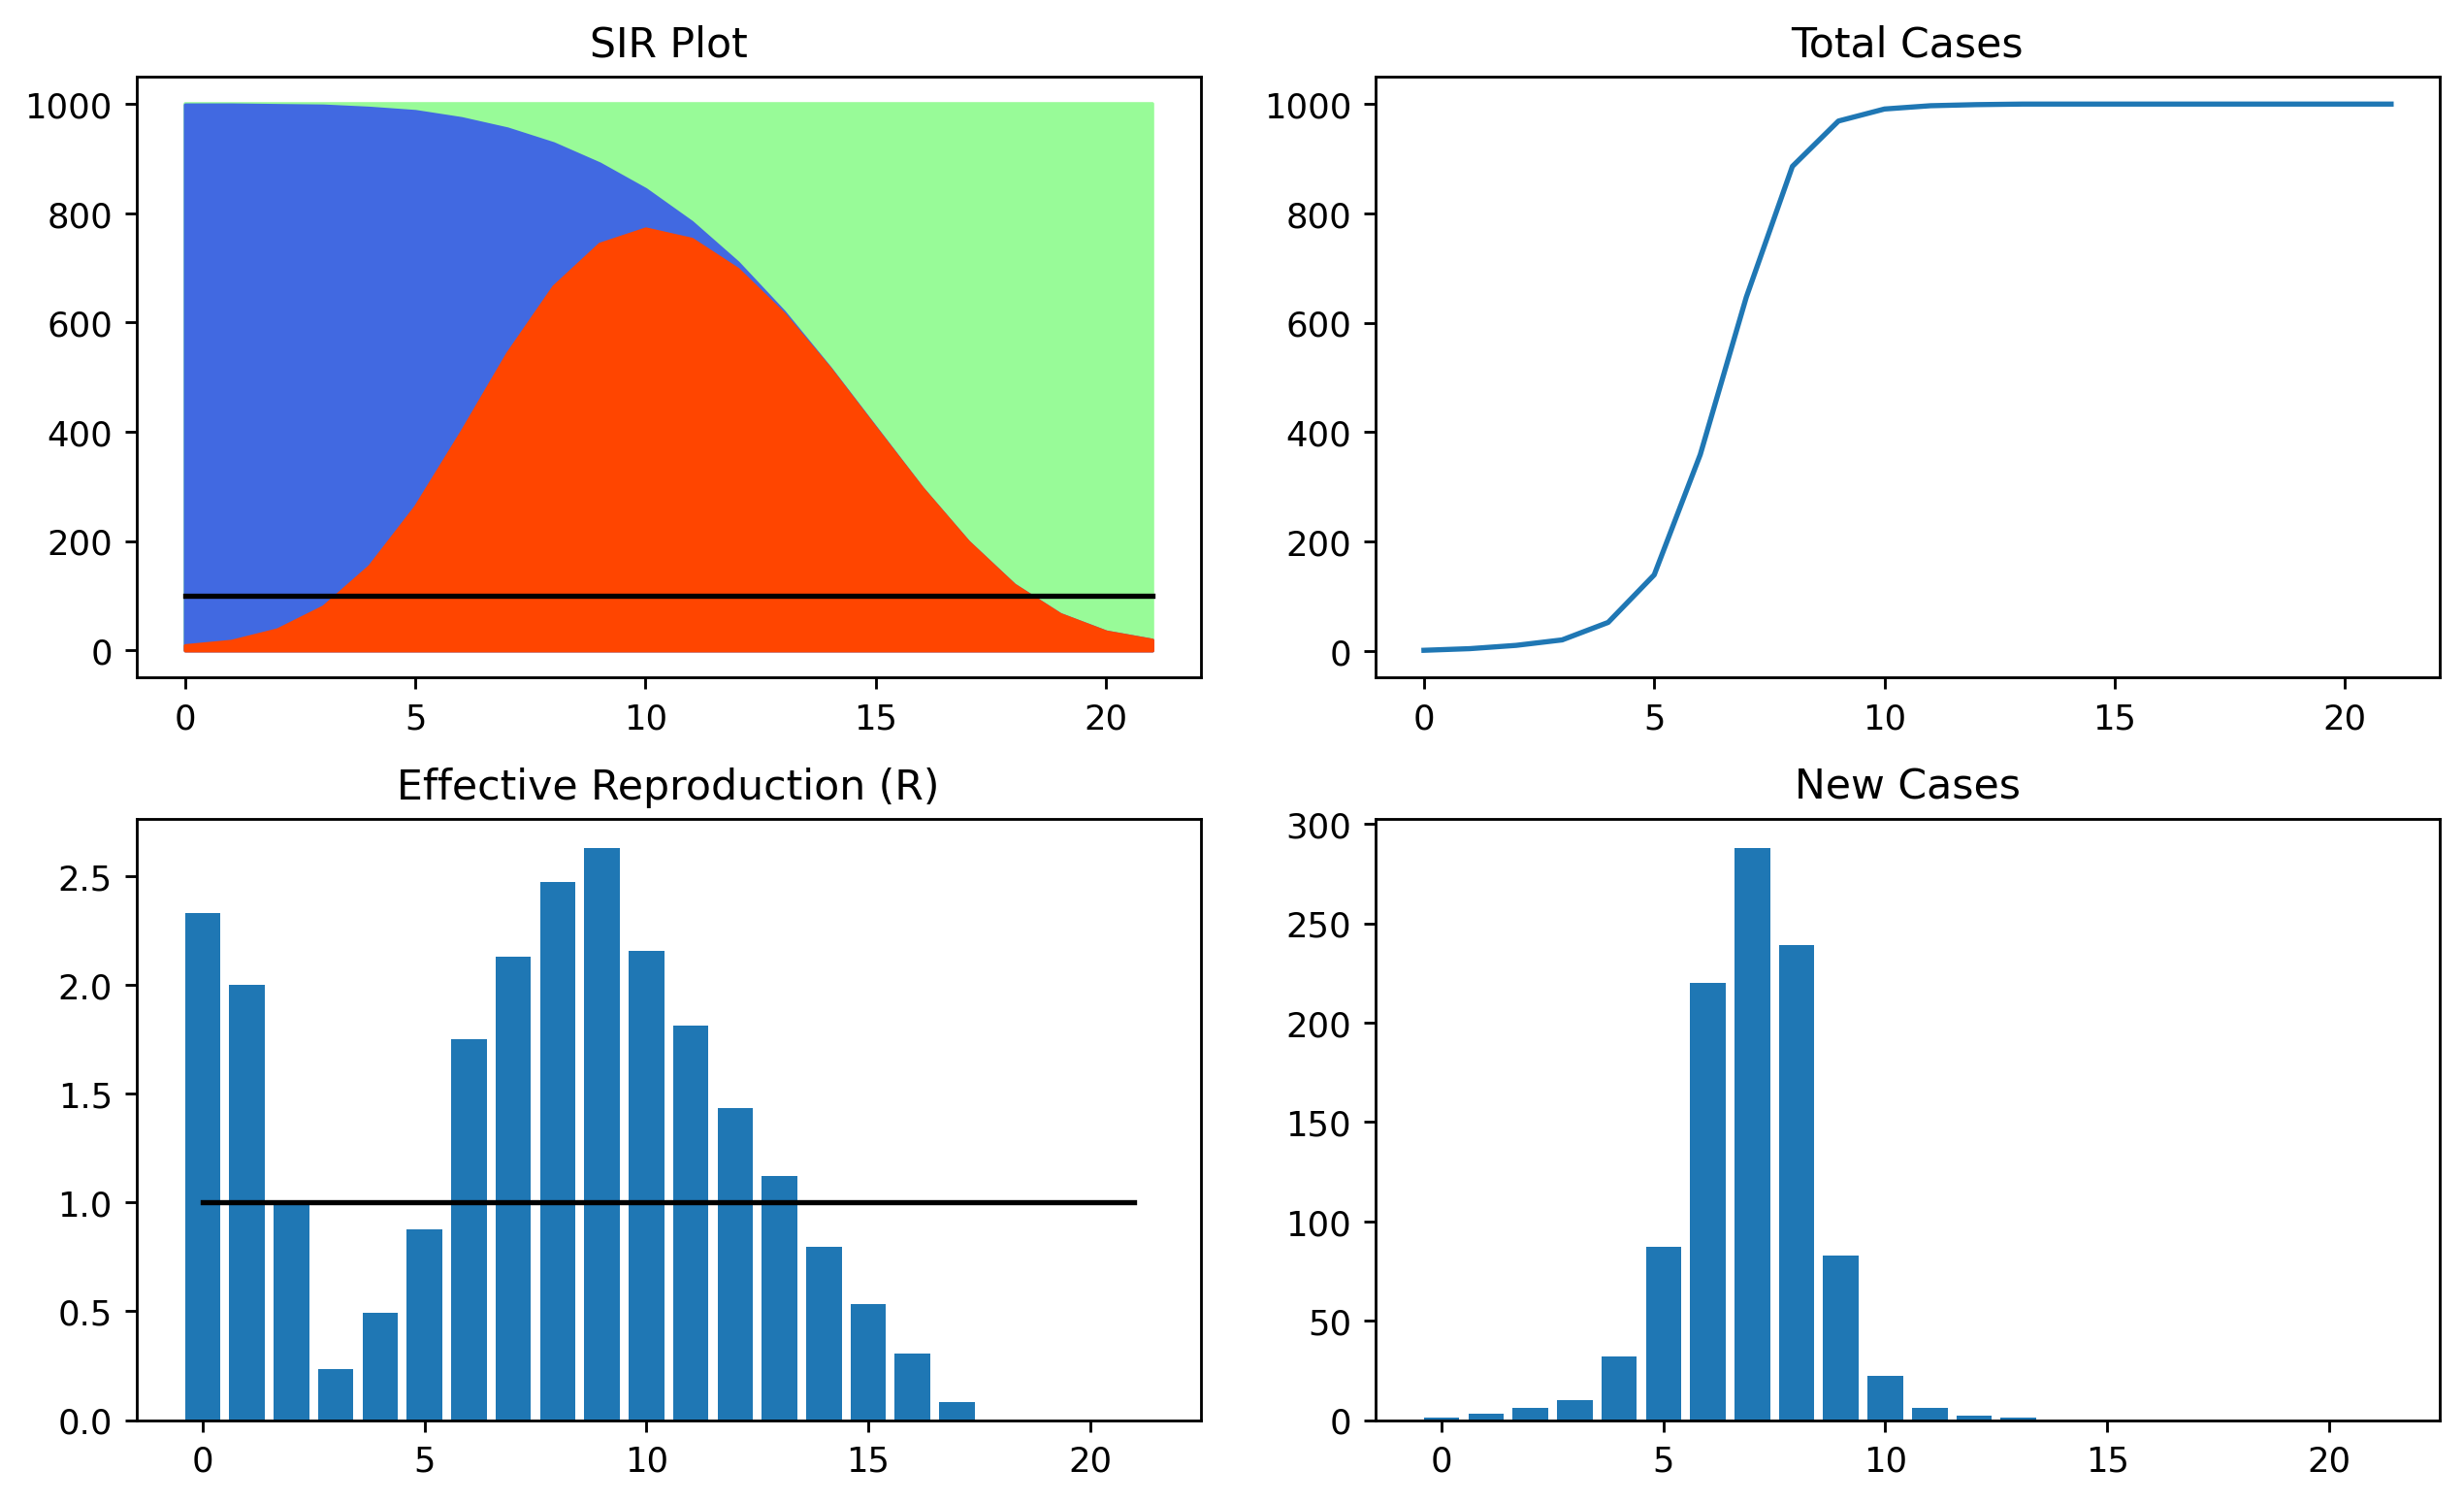
\includegraphics[scale=0.34]{baseline.png}
        		\caption{Base-case statistics}
            \end{figure}
            \subsubsection{SIR plot}
                The number of susceptible, infected and recovered/removed people is represented over the whole duration of the epidemic. A colour scheme is selected to categorize the different group of population, blue for susceptible, red for infected and green for recovered / removed people.
            \subsubsection{Total number of cases plot}
                The total number of cases on each passing day during the epidemic is represented.
            \subsubsection{Effective reproduction (R)  plot}
                The value of R on each passing day is represented.
            \subsubsection{New cases plot}
                The occurrence of new cases on each day is represented for the duration of epidemic.\\
        \subsection{Analysis}
            When increasing the ``connectedness" of the graph by increasing community centre count to 100 and average friend count to 20, the total duration falls down to 17 days, but the peak cases rise to 940. This was no surprise. It can be said that the disease was encouraged to spread rapidly, and hence was over quickly. But of course, this is no solution to the problem. When it was tried to go to the opposite end and decrease the connectedness of the graph by having only 10 community centres and only 5 friends on average, it was once again the expected results. The peak cases comes down to 681, and total cases down to 977 (i.e. few people were unaffected). It still crossed the number of beds available though. The effective reproduction might seem counter intuitive at first peaking at almost 2.75, unlike the previous case where it didn't even reach 2.5. But on closer inspection, this is because the number of people causing secondary infections are lesser. What matters here is that during the rise in cases, it too was on an uptrend and was above 1, signalling the increase. When the cases peaked out, R started on a downtrend.
            \begin{figure}[!h]
        		\includegraphics[scale=0.34]{connectednessUp.png}
        		\caption{Community Centres = 100, Average Friend Count = 20}
            \end{figure}
            \begin{figure}[!htb]
        		\includegraphics[scale=0.34]{connectednessDown.png}
        		\caption{Community Centres = 10, Average Friend Count = 5}
            \end{figure}
            \newpage
            Next the travel parameters are changed, namely the travel probability and the travel strictness. With travel probability set to 0.9 and travel strictness at 0 i.e. no travel ban, there wasn't much difference from the baseline. The duration was the same and once again everyone was infected. Peak cases slightly decreased, although this can be dismissed as noise. It was also tried going the other extreme with a complete travel ban, and once again there was no major difference.
             \begin{figure}[!htb]
        		\includegraphics[scale=0.34]{highTravelProb.png}
        		\caption{Average travel probability = 0.9}
            \end{figure}
            \begin{figure}[!htb]
        		\includegraphics[scale=0.34]{noTravel.png}
        		\caption{Travel ban strictness = 1}
            \end{figure}
            
            So why didn't the situation get drastically worse with everyone travelling? This was because the model had considered the population to be one giant cluster, without any smaller ``sub clusters". As a result there was no effect if people travelled or not. It's too late to go back and change the graph structure in code, but that's fine as we've got plenty of other parameters to work with.\\
            
            Average Social distance is the measure in meters between 2 nodes. This is used to determine the physical distance between two nodes which is the sum of average social distance and social distance variation, this physical distance will be one of the parameter to decide whether an adjacent node can be infected or not since if this physical distance is larger than the infection radius the disease cannot be transmitted. From this it can be easily concured that on increasing the average social distance between nodes, less nodes will be infected. As is visible in the graph, if increasing the average social distance to 2.2 from the base value of 1.25 it was seen in the SIR graph that the susceptible population is less than the base graph. Also the new cases graph is more spread out which means more time is taken for spreading of the infection.\\
            \begin{figure}[!h]
        		\includegraphics[scale=0.45]{avgsocialdist2.2.PNG}
        		\caption{Average Social Distance = 2.2}
            \end{figure} 
    
            Next consider a simulation of a scenario where the vaccination drive is in full swing causing the immunity to go up, and naturally people are following a less stricter quarantining. No doubt, it is observed that peak cases drops with considerable number of people remaining unaffected, but the disease is prolonged. While it might not look great initially to have the disease prolonged, it also helps make sure most people get the beds they need leading to a lower mortality rate.
            \begin{figure}[!htb]
        		\includegraphics[scale=0.35]{avgimmu.PNG}
        		\caption{Average immunity = 0.8, Quarantine Strictness = 0.5}
            \end{figure}
            
            To see whether contamination between two nodes is possible or not it has to be seen how many physical contacts a particular node makes. For this, there's a parameter called average physical contact between 2 nodes per day. For these physical contacts it is checked whether infection is possible between nodes considering other parameters also like immunity, quarantine probability etc. But ion keeping other parameters constant, it can be said that if the average number of physical contacts increase the infection will spread faster, as is visible in the graph below where the average physical contact has been increased to 20 from base value.\\
             \begin{figure}[!h]
        		\includegraphics[scale=0.45]{avgphysicalcontact20.PNG}
        		\caption{Average number of physical contact between 2 people in a day = 20}
            \end{figure}
    
    As depicted above, increasing the average physical contacts increase the infection rate in the population. But it is known that many other factors are also working for determining the infection rate like on increasing the average physical contact to 20 as shown above but with that there should be an increase in the average immunity of the population as well, say, to 0.8 from base value of 0.2, it's seen that although more people are coming in contact, since the immunity is increased the chance getting infected gets decreased. In the graph below it can be seen the new cases graph is more spread out and in the SIR graph also the increase in susceptible cases is not sudden whereas it increases slowly.\\
    \begin{figure}[!h]
		\includegraphics[scale=0.45]{avgphysicalcontact20avgimmunity0.8.PNG}
		\caption{Average number of physical contact between 2 people in a day = 20 average immunity = 0.8}
    \end{figure}
    
    Quarantine Strictness - It represents the scale(0 to 1, 0 being the lowest, i.e no strictness) of strictness followed when a infected person is quarantined. At the baseline level this research has kept quarantine strictness high which is quite likely in real scenario. But if on changing it from 0.9 to 0.15, it can be observed that the disease takes more time to eradicate and also the peak number of cases is reached in less time.\\
    \begin{figure}[!h]
		\includegraphics[scale=0.45]{strictness.PNG}
		\caption{Quarantine strictness = 0.15}
    \end{figure}
    
    Quarantine Probability - It represents the probability of an infected person to be quarantined. For the baseline, this research has taken quarantine probability to be 0.25. Changing it to 1, i.e if everyone being affected is quarantined, it is observed that number of peak cases is dropped and a few people are not affected at all. It is also observed that it takes more time for the disease to eradicate. On the other hand if quarantine probability is set to 0, it is observed that, the whole population is affected in less duration of time and peak number of cases is also increased.
    \begin{figure}[!h]
        		\includegraphics[scale=0.43]{probability1.PNG}
        		\caption{Quarantine probability = 1}
    \end{figure}
    \begin{figure}[!h]
        		\includegraphics[scale=0.43]{probability2.PNG}
        		\caption{Quarantine probability = 0}
    \end{figure}
    
    The following graphs show the effect of increasing the number of hospital  beds and ensuring those get occupied more often than not.\\
    \begin{figure}[!h]
		\includegraphics[scale=0.33]{bed probability.PNG}
		\caption{Beds available = 800, Quarantine Probability = 0.8}
    \end{figure}
    
    As baseline, the number of available beds (hospital beds) is sufficient for 10\% of the total population. If it is increased to 80\%, it is observed that disease doesn't affect the whole population, but there is no considerable changes in peak, daily new cases etc. This is due to the fact that there is an increase in the number of hospital beds but the probability of quarantining infected people is still low (0.25). On increasing that to 0.8, a drastic change occurs, the graphs flattens considerably, with less number of daily cases.\\
    
    Average duration of infection - It is the period (in days) that the infection affects the infected. This research has taken the base degree for this variable as 9. But when it is increased to 25, certain changes can be seen in the graphs. The total epidemic duration increased to 38, but the peak cases remains nearly the same.
    \begin{figure}[!h]
		\includegraphics[scale=0.45]{1-Average duration.png}
		\caption{Average duration of infection = 25}
    \end{figure}
    
    \vspace{0.1in}
    Summarizing the key observations:
    \begin{itemize}
        \item The trivial way to get out of an epidemic is to simply not take any care and have everyone infected. This of course is not the solution as it leads to several deaths.
        \item With increase in the number of community centres, there was a rapid increase in the number of cases per day, so less human gathering equals better epidemic control.
        \item With increase in the average distance among people, i.e maintaining social distance, the chances of disease spreading can be reduced.
        \item Once vaccinated, people can start engaging in social activities and gatherings as they would be immune. Quarantine strictness can also be relaxed.
        \item Quarantine strictness is also very important as even with 100\% quarantining, if there is a lack of strictness, then the disease will spread. That said, if both are taken care of, it helps significantly curb the disease.
        \item With increase in the number of hospitals beds and observing quarantine more strictly, the disease spread can be reduced significantly.
    \end{itemize}
         
    \section{Conclusion}
        Having analysed the simulation results and drawn necessary conclusions, this research can now formally wrap everything up. The research started with identifying the problem statement and laying out the requirements. With that done, this research then went through the literature available, to gain valuable insights to help along the way. It was also discovered that what this research had planned to do, while wasn't unexplored territory, also wasn't done in the way this research had planned to. Therefore the research plan was finalised, thus began the simulation software development phase. Once that was nearing its end, the testing and analysis phase was started, which was followed up with the final documentation phase.\\

        The said simulation software used a modified BFS to spread the disease. Unlike in the traditional BFS, the nodes were retained in the queue until their status changed to `Removed'. The queue was also shuffled each time to randomise the spread. During the analysis phase, the input parameters were tweaked to analyse different scenarios, and it was proved empirically the significance of the different measures one can take to help minimise the spread and "flatten the curve".\\

        While this has done a significant work, both in terms of the software development and simulation analysis, there will always be ways to build upon and improve this research. For anyone wanting to take over from this point of the research, the suggestion is to start by restructuring the graph to incorporate the travel parameters effectively. This was something this research had failed to do. Then they can also think of other parameters to include to more generalise the simulation to other diseases. If further interested, they can consider modelling the spread of diseases over different climatic conditions. We're sure the more one would build on this research, the more opportunities and ideas he / she would come up with.
        
    \vspace{0.1in}
    \section{Applications}
        \begin{itemize}
            \item Identifying the critical parameters that contribute the most to the spread of contagions. In other words one can identify what measures can be the most helpful in containing the spread of disease.
            \item Spreading awareness among people and the government about the necessary measures to be taken for handling the spread of the epidemic.
            \item In the event of a future pandemic, the various critical parameters according to the situation then as well as the properties of the new contagion, can be deduced.
            \item Identify the measures that can be taken to minimise economic losses, while still containing the disease.
        \end{itemize}

    \section{References}
    \begin{enumerate}
        \item Zhao, P. (2020). A Social Network Model of the COVID-19 Pandemic. Retrieved from \url{https://doi.org/10.1101/2020.03.23.20041798}.
        
        \item Zaplotnik, Z., Gavrić, A., \& Medic L. (2020). Simulation of the COVID-19 pandemic on the social network of Slovenia. Retrieved from \url{https://journals.plos.org/plosone/article?id=10.1371/journal.pone.0238090}.
        
        \item Cherry, J., Krogstad, P. (2004). SARS: The First Pandemic of the 21st Century. Retrieved from \url{https://doi.org/10.1203/01.PDR.0000129184.87042.FC}
        
        \item Ferguson, N., Cummings, D., Cauchemez, S. et al. (2005). Strategies for containing an emerging influenza pandemic in Southeast Asia. Retrieved from \url{https://doi.org/10.1038/nature04017}
        
        \item Jiang, S., Wang, K., Li, C. et al. (2017). Mathematical models for devising the optimal Ebola virus disease eradication. Retrieved from \url{https://doi.org/10.1186/s12967-017-1224-6}
        
        \item Bansal, S., Grenfell, B. \& Meyers, L. (2007). When individual behaviour matters: homogeneous and network models in epidemiology. Retrieved from \url{https://doi.org/10.1098/rsif.2007.1100}
        
        \item Chao, D., Halloran, E. et al. (2010). FluTE, a Publicly Available Stochastic Influenza Epidemic Simulation Model. Retrieved from \url{https://doi.org/10.1371/journal.pcbi.1000656}
        
        \item Nguyen, D., Deguchi, H. et al. (2010). Agent-based simulation on avian influenza in Vietnam: Basic characteristics of the epidemic and efficiency evaluation of control measures. Retrieved from \url{https://ieeexplore.ieee.org/abstract/document/5530215}
        
        \item Tuite, A., Eisenberg, M. et al. (2011). Cholera Epidemic in Haiti, 2010: Using a Transmission Model to Explain Spatial Spread of Disease and Identify Optimal Control Interventions. Retrieved from \url{www.researchgate.net/publication/50304455}
        
        \item Nassar, M., Meo, S. et al. (2018). Global seasonal occurrence of Middle East Respiratory Syndrome Coronavirus (MERS-CoV) infection. Retrieved from \url{www.researchgate.net/publication/326041885}
        
        \item Hossain, M. et al. (2020). The effects of border control and quarantine measures on the spread of COVID-19. Retrieved from \url{www.sciencedirect.com/science/article/pii/S1755436520300244}
    
        \item Sanderson, G. (2020). Simulating an epidemic. Retrieved from \url{https://www.youtube.com/watch?v=gxAaO2rsdIs}
        
        \item Sanderson, G. (2020). Exponential growth and epidemics. Retrieved from \url{https://www.youtube.com/watch?v=Kas0tIxDvrg}
        
        \item Iyengar, S. (2019). Social Networks. Retrieved from \url{https://www.youtube.com/playlist?list=PLyqSpQzTE6M8CLBcLnq-f3vHRH-klC39L}
        
        \item Stevens, H. (2020). Why outbreaks like coronavirus spread exponentially, and how to “flatten the curve”. Retrieved from \url{https://www.washingtonpost.com/graphics/2020/world/corona-simulator}.
        
        \item Simler K. (2020). Outbreak. Retrieved from \url{https://meltingasphalt.com/interactive/outbreak}.
    \end{enumerate}
\end{document}